\documentclass{article}
\DeclareMathSizes{10}{10}{7}{7}
\usepackage{amsmath}
\usepackage{ amssymb }
\usepackage{tikz, graphicx}
\usepackage{geometry}
\usepackage[makeroom]{cancel}
\usepackage[export]{adjustbox}
\DeclareMathOperator{\sech}{sech}
\usepackage{subfig}
\usepackage[framed,numbered,autolinebreaks,useliterate]{mcode}
\usepackage{hyperref}
\hypersetup{
    colorlinks=true,
    linkcolor=blue,
    filecolor=magenta,      
    urlcolor=blue,
    }
\usepackage{float}
\restylefloat{table}

\geometry{legalpaper, margin=0.7in}

\title{3AN Project 2\\ What happened when two waves crossed the glass road}
\author{Liam Watson WTSLIA001}
\begin{document}
\maketitle
\section{Introduction and physics}
We wish to better understand the interaction between colliding solitons within some optical communication media such as fibre optic cable used for audio or network communications. 
We can model optical pulses in a media with saturation non-linearity properties using the following modified nonlinear  Schrodinger equation:
\begin{align}
i\psi_t + \psi_{xx} + \frac{2|\psi|^2\psi}{1+S\sin(|\psi|^2)} = 0
\end{align}
Note that we impose periodic boundary conditions to the Schrodinger equation. \\
We can study the collisions of N solitons by choosing our initial configuration as the sum of N solitons separated by a sufficiently large distance as follows:
\begin{align}
\psi (x,0) = \sum_{j=1}^N A_j \sech(A_j (x-x_j))e^{iv_j(x-x_j)}
\end{align}
For this paper we will consider only the case of $N=2$.\\
In the following sections we will study soliton collisions for different values of the non-linearity saturation $S\in(-1,1)$, the velocity $v_{1,2}$ and the intersoliton distance $|x_k-x_j|$. \\
This analysis will be done using two different numerical methods, namely the Split-Step and Finite Difference methods. To ensure that any insight gained from either method is consistent we will ensure that the following conserved quantity remains within a maximum deviation of $\varepsilon = 10^{-4}$.
\begin{align}
D = \int_{-\infty}^\infty |\psi|^2 dx
\end{align}
Additionally we will compare the execution time of both numerical methods for the given $\varepsilon$.
\section{Presentation of needed numerical method formula}
In the following two sections we will discuss the derivation of the formula needed for the implementation of the two numerical methods. 
\subsection{Split-Step}
The Split-step method relies on splitting the differential equation (1) into a nonlinear part and using it to solve the linear part. After some intermediate steps we find that the nonlinear part can be expressed as
\begin{align}
\psi = \psi(x,0) e^{\frac{2iCt}{1+S\sin(c)}},\text{\ \ \ } C = |\psi|^2
\end{align}
Note that we know $C$ is constant as 
\begin{align}
\psi_t \bar{\psi} + \bar{\psi_t} + \psi = 0 \implies \frac{\partial}{\partial t}(\psi\bar{\psi}) = 0 \implies |\psi|^2 = C
\end{align}
We move onto the linear part which after using a Fourier series expansion over our discretized region can be expressed by
\begin{align}
W(x,t_{k+1}) = \sum_{-N/2}^{N/2-1} W_k e^{\frac{2 \pi i k x}{L}}
\end{align}
\subsection{Finite Difference}
There are three main methods that we can use for a finite difference expansion namely, Explicit, Implicit and Crank Nicolson. \\
Crank Nicolson method produces the following expression for (1) after discretizing in time and space and substituting in the relevant approximations. 
\begin{align}
i\psi_{j,k+1} + \frac{\tau}{2h^2}(\psi_{j-1,k+1} -2\psi_{j,k+1} + \psi_{j+1,k+1}) = i\psi_{j,k} - \frac{\tau}{2h^2}(\psi_{j-1,k}-2\psi_{j,k} + \psi_{j+1,k}) - \frac{2\tau |\psi|^2 \psi}{1+S\sin|\psi|^2}
\end{align}
From the above equation we can formulate a matrix vector equation to solve for $\psi_{j,k+1}$. Note that we use the periodic boundary conditions in our matrix to fill in values needed for a center difference approximation. (See lines 29 and 30 of code in section 3.2). There is no need to write more here as the relevant information is more explicitly covered in the code section 3.2.
\section{Implementation}
In the following two sections the implementation will be briefly discussed with code following. Note that a detailed explanation of each line is left as a comment in the code blocks. The code can be found on \href{https://github.com/Liam-Watson/SolitonColisonsInOpticalFiber}{github} if needed. 
\subsection{Split-Step}
The general procedure followed here is a follows
\begin{enumerate}
\item Define spacial and temporal region and mesh
\item Define the initial two soliton's with amplitude [A1,A2], velocity [v1,v2], intial position [xPos1,xPos2] and saturation of non-linearity $S$.
\item At each itteration (time step) update psi using the update formula and the Fast Fourier Transform and (inverse) schemes. 
\item Plot reults at each time step and plot 3D at the end of the simulation. 
\end{enumerate}
\begin{lstlisting}
clear all; %Ensure testing is not effected by past computation
clc;

L = 100; %Simulation space interval
N = 1000; %Number of mesh points
h = L/N; %Size of mesh spacing
x = 0:h:(L-h); %Discretized spacial interval
tau = h^2/3;%The method is explicit so there is a stability condition
A1 = 1; %Aplitude of soliton 1
A2 = 1; %Aplitude of soliton 2
S = 0.9; %Saturation of nonlinearity
xPos1 = 30;  %Starting position of wave peak in x direction
xPos2 = 60; %Starting position of wave peak in x direction
v1 = 1;  %Velocity of soliton 1
v2 = -1; %Velocity of soliton 1
psi = A1*sech(A1*(x-xPos1)).*exp(1i*v1*(x-xPos1))...%Soliton 1 Inital
      + A2*sech(A2*(x-xPos2)).*exp(1i*v2*(x-xPos2));%Soliton 2 Inital
plot(x,abs(psi))%Plot inital configuration. Removed for testing speed
time=3000; %Max time. This value will vary across testing.

%Used for 3D plot. Removed for testing
X = [x];
Y = [abs(psi)];
Z = [0:time];
%%%%%%%%%%%%%%%%
vecTmp = 4*pi^2/L^2*[0:N/2 - 1 -N/2:-1].^2; %Intermediate simplification needed in line 29
for ti=1:time
    psi = psi.*exp((tau*2.i*abs(psi).^2)./(1+S*sin(abs(psi).^2))); %Update psi
    psi = ifft(fft(psi).*exp(-1i*tau*vecTmp)); %Update psi with FFT and IFFT approxmiation
    Const = trapz(x,abs(psi).^2); %The conserved quantity

    Y = [Y;abs(psi)]; %Used for 3D plot. Removed for performance testing
    
    plot(x,abs(psi)), drawnow %Plot 2D updated solution for time t. Removed for performance testing
end

h = surf(X,Z,Y) %Plot 3D, x, t, psi 
set(h,'LineStyle','none') %Set the mesh lines to not display as the mesh is too dense
end
\end{lstlisting}
\pagebreak
\subsection{Finite Difference}
The general procedure is as follows:
\begin{enumerate}
\item Define spacial and temporal region and mesh
\item Define the initial two soliton's with amplitude [A1,A2], velocity [v1,v2], intial position [xPos1,xPos2] and saturation of non-linearity $S$.
\item Define the matrix A needed for solving the matrix vector equation. 
\item Find the inverse of A
\item Define the RHS vecotr needed for solving the vector matrix equation according to the update formula
\item Solve the vector matrix equation and update psi with the new numerical solution
\item Plot reults at each time step and plot 3D at the end of the simulation. 
\end{enumerate}
\begin{lstlisting}
clear all; %Ensure testing is not effected by past computation
clc;

L = 100; %Overall simulation interval
N = 3000; %Number of space subdivisions
h = L/N; %Size of mesh spacing
x = [0:h:(L-h)]'; %Space mesh
tau = h^2/3; %Time step

A1 = 1; %Inital amplitude of soliton 1
A2 = 1; %Intial amplitude of soliton 2
S = 0.0; %Nonlinarity saturation
xPos1 = 30; %Starting position of wave peak in x direction
xPos2 = 60; %Starting position of wave peak in x direction

v1 = 1; %Velocity of soliton 1
v2 = -1; %%Velocity of soliton 2
psi = A1*sech(A1*(x-xPos1)).*exp(1i*v1*(x-xPos1))...%Soliton 1 Inital
      + A2*sech(A2*(x-xPos2)).*exp(1i*v2*(x-xPos2));%Soliton 2 Inital

plot(x,abs(psi)) %Plot inital configuration. Removed for testing speed

s = tau/h^2; %code simplifcation
s2 = s/2; %code simplifcation

A = diag((1i-s)*ones(N,1),0)... %Set the FD matrix values on diagonals
    +diag(s2*ones(N-1,1),1)...
    +diag(s2*ones(N-1,1),-1);
A(1,N) = s2; %Set periodic BC elements in matrix A
A(N,1) = s2; 
A = inv(A); %Performance enhancement change referenced in section 4.1
rhs = zeros(size(x)); %Create RHS vector. Performance enhancement change referenced in section 4.1
time = 3500; %Max time. Can change depending on needed time interval

X = [x]; %Used for 3D plot. All removed for performance testing. 
Y = [abs(psi)];%Used for 3D plot
Z = [0:time];%Used for 3D plot
for t=1:time %Loop until max time reached   
    rhs(2:N-1) = (1i + s)*psi(2:N-1)-s2*psi(1:N-2)... %Update RHS
        - s2*psi(3:N)...
        - (2*tau*(abs(psi(2:N-1)).^2).*psi(2:N-1))./(1+S*sin(abs(psi(2:N-1)).^2)); %CN approxmiation
        %- (tau*(abs(psi(1:N-2)).^2).*psi(1:N-2))./(1+S*sin(abs(psi(1:N-2))))...
        %- (tau*(abs(psi(3:N)).^2).*psi(3:N))./(1+S*sin(abs(psi(3:N))));
        
    
    rhs(1) = (1i + s)*psi(1) -s2*psi(2) -s2*psi(N)...
        -(2*tau*abs(psi(N)).^2.*psi(N))/(1+S*sin(abs(psi(N)).^2)); %CN approxmiation
        %-(tau*abs(psi(N)).^2.*psi(N))/(1+S*sin(abs(psi(N))))...
        %-(tau*abs(psi(2)).^2.*psi(2))/(1+S*sin(abs(psi(2))));
        
    
    rhs(N) = (1i + s)*psi(N) -s2*psi(1) -s2*psi(N-1)...
            -(2*tau*abs(psi(N)).^2.*psi(N))/(1+S*sin(abs(psi(N)).^2)); %CN approxmiation
            %Both implicit and explicit methods were attempted to see if they could integrate better. See section 4.1. 
            %-(tau*abs(psi(N-1)).^2.*psi(N-1))/(1+S*sin(abs(psi(N-1))))... 
            %-(tau*abs(psi(1)).^2.*psi(1))/(1+S*sin(abs(psi(1))));
    %psi = A\rhs; %Removed for performance reasonsons. See line bellow. 
    psi= A*rhs; %Solve for psi
    Y = [abs(psi) Y]; %%Used for 3D plot. Removed for performance testing.
    Const = trapz(x,abs(psi).^2); %The conserved quantity. Removed for performance testing.
    
    plot(x,abs(psi)), drawnow %Plot 2D updated solution for time t
end

h = surf(X,Z,Y') %Plot 3D, x, t, psi
set(h,'LineStyle','none')
end
\end{lstlisting}
\pagebreak
\section{Results and Discussion}
\subsection{Performance and accuracy}
We choose $S=0$, $v_1 = 1$, $v_2 = -1$, $x_1 = 30$, for the following testing. 
In order to test both methods performance we must calibrate the two methods hyper-parameters so that the conserved quantity deviation is less than $\varepsilon = 10^{-4}$ (the best achievable with computing and memory requirements). We find after some initial testing that the Finite Difference method deviates more than the Split Step method for any given mesh spacing. This is likely due to the nonlinear Schrodinger equation not being integrable. The Split Step method avoids this as both the linear and nonlinear parts are integrable where as the Finite Difference method attempts to directly solve the equation (1). \\
Calibration results in the following choices of parameters for testing. \\
Finite Difference: $N=2000$ and $\tau = h^2/3 = 8.333\cdot 10^{-4}$ \\
The resulting conserved qunatity near the collision is $4.000089807509760$.\\
Since $\tau$ is linked to the choice of $N$ we must choose the same $\tau$ for the Split Step method. \\
Split Step: $N=150$ and $\tau = 8.333\cdot 10^{-4}$. The resulting conserved qunatity is approximately $4.000088112839693$\\
Both values are within the specified deviation $\varepsilon$ as the expected value is $4$.\\
The testing was completed using Matlabs tic toc routine with timing starting before any variable assignment and after $6000$ time steps (at the end of the simulation). 
We ensure consistency by removing all plotting routines and their required variables and printing routines. Additionally, we clear all cached data.\\
Run time analysis:\\
Split Step: Elapsed time is 0.256348 seconds.\\
Finite Difference:  Elapsed time is 3416.665484 seconds. This is a very poor result which can be improved with some optimization of memory by declaring vectors before hand using the zeros routine and calculating the inverse of our $A$ matrix once before the loop rather than every iteration. Which results in a elapsed time of 51.400328 seconds. Which is better but still poor given the fairly high $\varepsilon$.

\subsection{Analysis of numerical solutions}
\begin{enumerate}
\item

The performance of the Finite Difference method is very poor. So first let us verify that both schemes produce similar results at least qualitatively so that we can assume that results that hold for split step will be applicable to the Finite Difference method. Note that in some cases for large values of nonlinear saturation the Finite Difference method fails completely unless the simulation granularity is very large which was attempted but after over six hours of simulation it was decided that this was the best solution. The failed simulation saw massive deviation in the conserved quantity as well as many ripples forming around the solitions after just a few time steps which is not a physicaly based phenomenon. \\
A note on interpreting heat maps: The more red shifted the pixel value the larger the $\psi$ amplitude at any given spacial and temporal coordinate. We use heat maps as they allow us to better see the effects of various changes in parameters over time without excessive use of 2D images or video formatts. 

\begin{figure}[h!]

\title{Finite difference method solution to equation (1)\\}
%\centering
\includegraphics[scale=0.3]{Capture.PNG}
\caption{\\The above figure is the solution of equation (1) using the Finite Difference method over 6000 time steps, $N = 2000$, $v_1=-v_2= 1$, $x_1=30$, $x_2=60$ and $S=0.5$. We can verify that this is the same result, qualitatively, that is produced by the split step method as seen in figure 2 bellow. }
\end{figure}


\begin{figure}[h!]
\title{Split Step method solution to equation (1)\\}
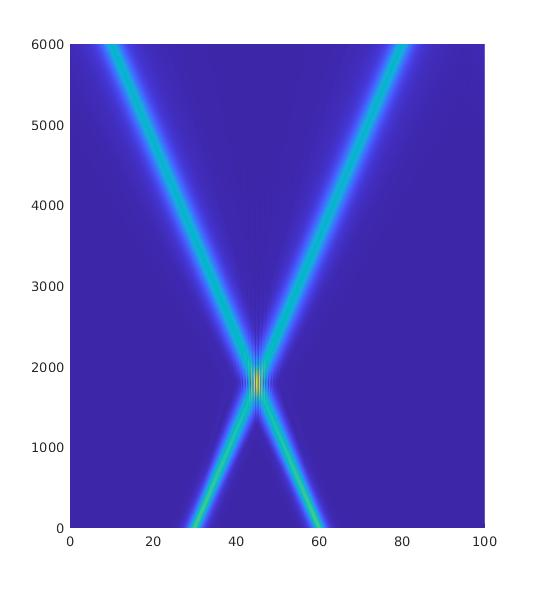
\includegraphics[scale=0.4]{Capture3.jpg}
\caption{As we can see the qualitative properties of the solutions are the same with split step being more computationally efficient and accurate as the conserved quantity does not vary more than $\varepsilon=10^{-12}$ with an $N=2000$ in this test.}
\end{figure}
\pagebreak
\begin{figure}[h!]
\title{Figure 1 from a different perspective.\\}
\includegraphics[scale=0.32]{Capture2.PNG}
\caption{\\Here we can see that the qualitative properties of the solitons are best captured by a heat map. However, it is included to better demonstrate the amplitude of the solitons as well as the "interference patterns" caused by the non-linearity.}
\end{figure}
From the above Figures 1,2 and 3 we can see that qualitative results are equivalent for both numerical methods hence all figures from this point will be produced using the superior Split Step method which performs better in all quantitative measures. 
\pagebreak
\item Testing small and large velocity \\
To keep testing consistent the following figures were obtained with $N=1000$ due to memory and processor restrictions. The maximum time was allowed to vary as was needed for the various velocities. 
\begin{figure}[h!]
\title{Soliton heat maps for various velocities for $S=0$\\}

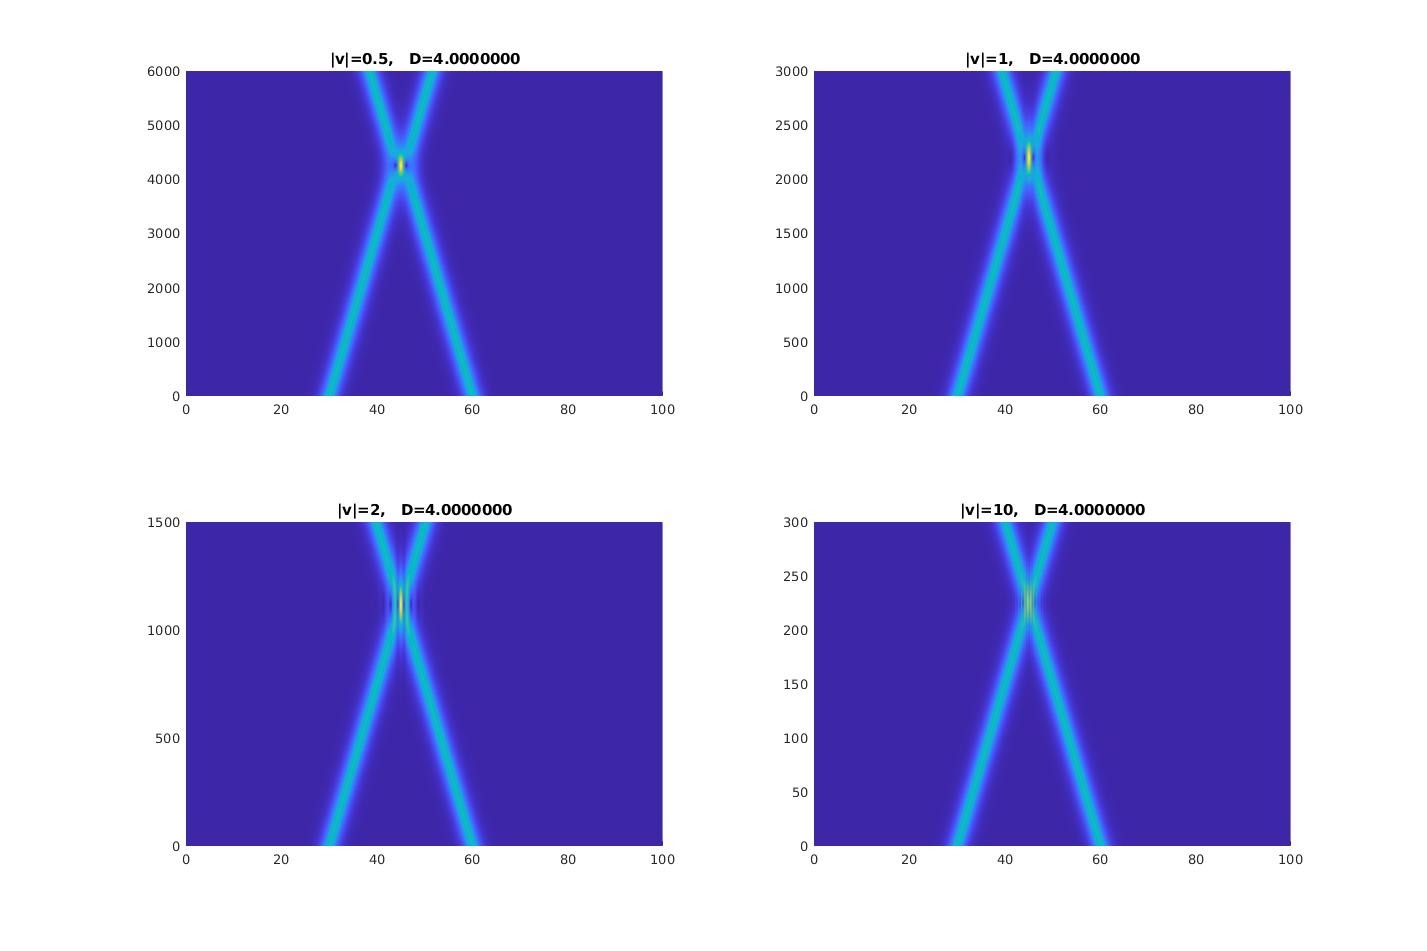
\includegraphics[scale=0.35,center]{3D_V_S0.jpg}
\caption{We can see that for small velocities 0.5 and 1 there is no unexpected behavior, the waves collide (adding amplitudes) and separate without any secondary effects. As the velocity increases we start to see many large amplitude spikes that then separate without any secondary effects. Additionally, the collision is elastic with the solitons having a constant amplitude before and after the collision.}
\end{figure}
%\pagebreak
\begin{figure}[h!]
\title{A different angle for figure 4\\}
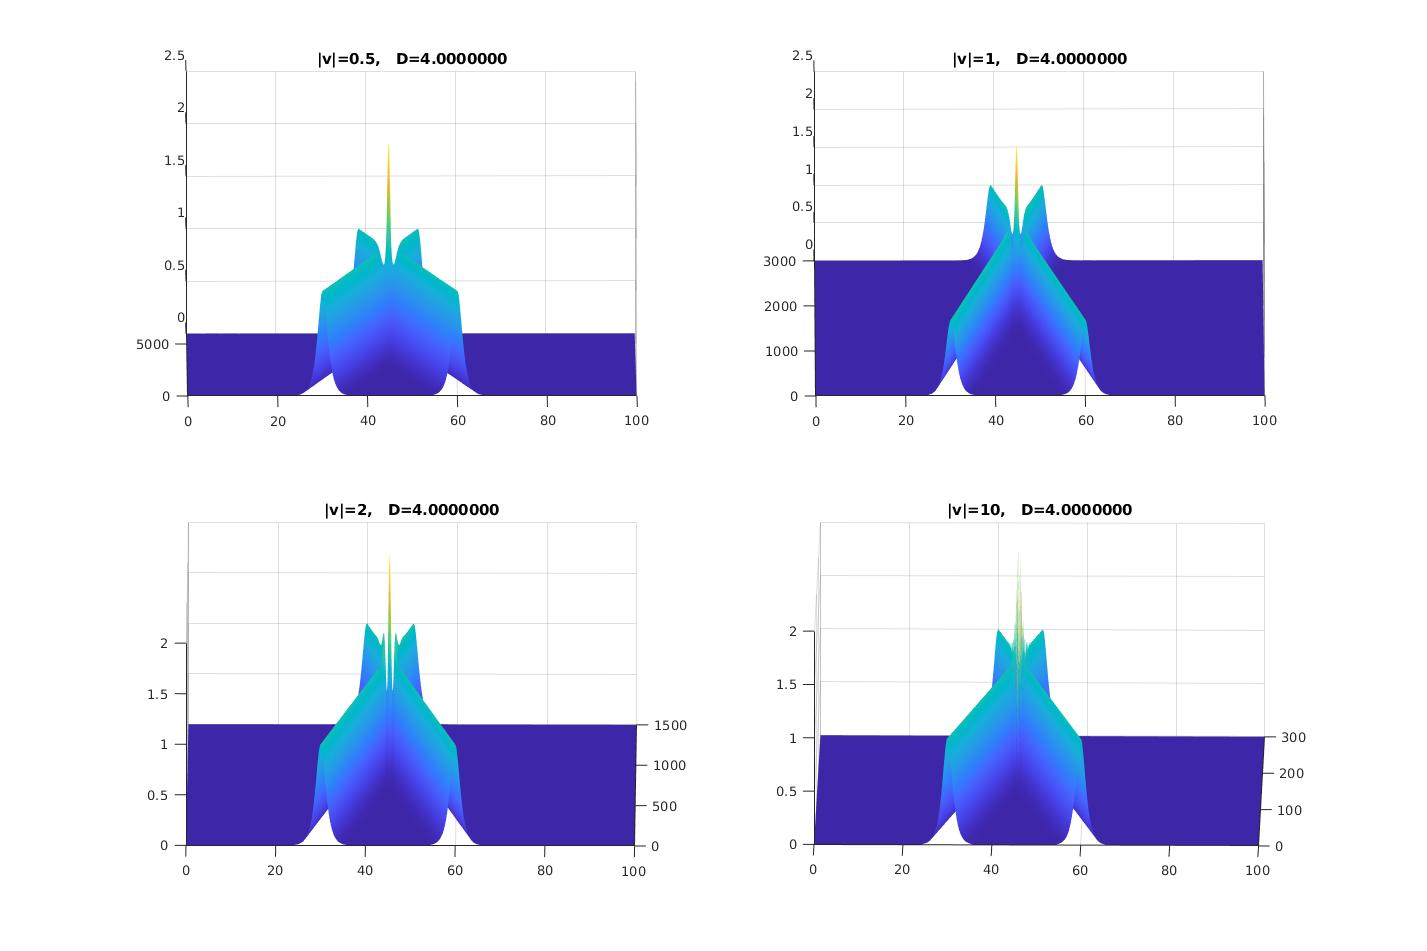
\includegraphics[scale=0.24,center]{3D2_V_S0.jpg}
\caption{We include this figure to demonstrate more clearly the "spikes" at the collision of the two solitons for large velocities}
\end{figure}

The result with zero non-linearity is uninteresting with expected results apart from the spikes forming at the intersection of the two solitons. Let us now investigate positive non-linearity $S$. \pagebreak
\pagebreak
\begin{figure}[h!]
\title{Soliton heat maps for various velocities for $S=0.5$\\}
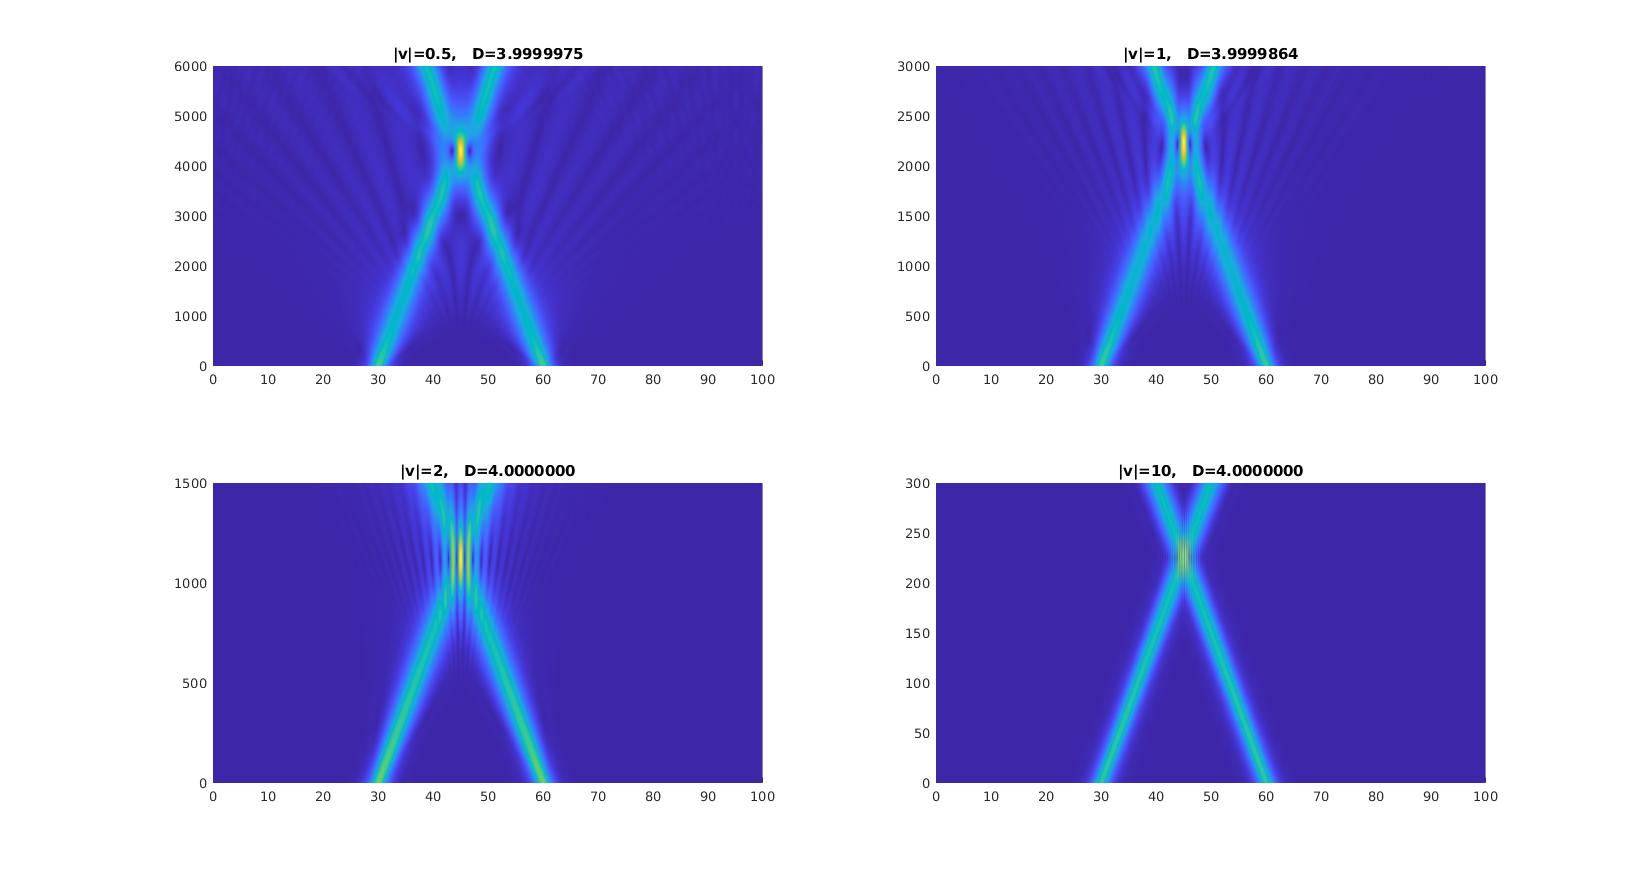
\includegraphics[scale=0.32,center]{3D_V_S05.jpg}
\caption{We can see that waves of smaller amplitude are produced for small velocities which decrease as we increase velocity.}
\end{figure}
\begin{figure}[h!]
\title{Soliton heat maps for various velocities for $S=0.9$\\}
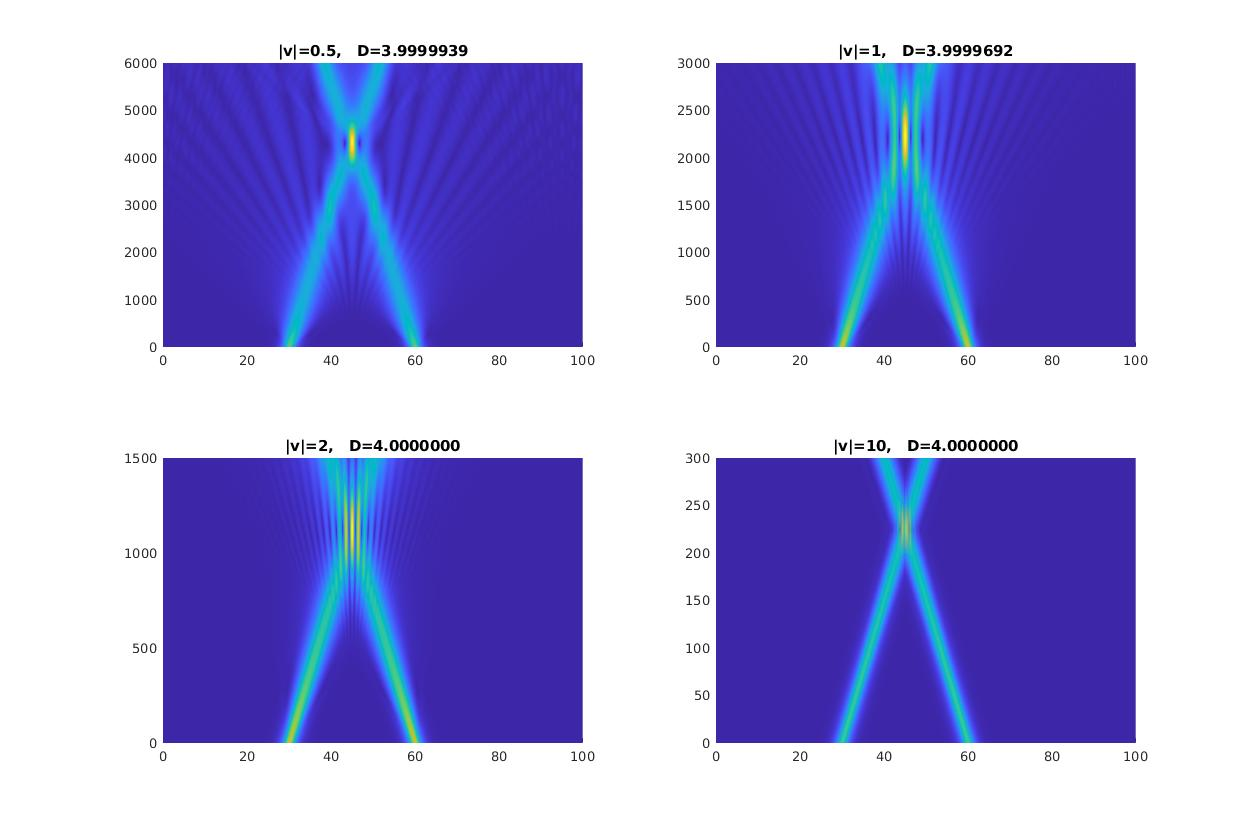
\includegraphics[scale=0.35,center]{3D_V_S09.jpg}
\caption{In the above figure we can see the same effect as in Figure 6, however, more pronounced}
\end{figure}
\begin{flushleft}
In figures 6 and 7 we can see unexpected formation of secondary waves that form before the collision of the two solitons and spread away from the intersection point. These secondary waves remove energy from the two initial solitons thus decreasing signal strength within the transmission medium. Additionally, these smaller waves may be interpreted as an intentional pulse to any receiver and thus we must be cautious with the sensitivity of the reciever when two soliton signals collide. \\
\end{flushleft}
\pagebreak
\item Negative nonlinearity \\
We know from before that phenomenon incurred by some value of non-linearity was emphasized by increasing saturation magnitude but not qualitatively changed given the sign is consistent (this was verified but not included in this paper for brevity) so we will only test $S = -0.9$.

\begin{figure}[h!]
\title{Soliton heat maps for various velocities for $S=-0.9$\\}
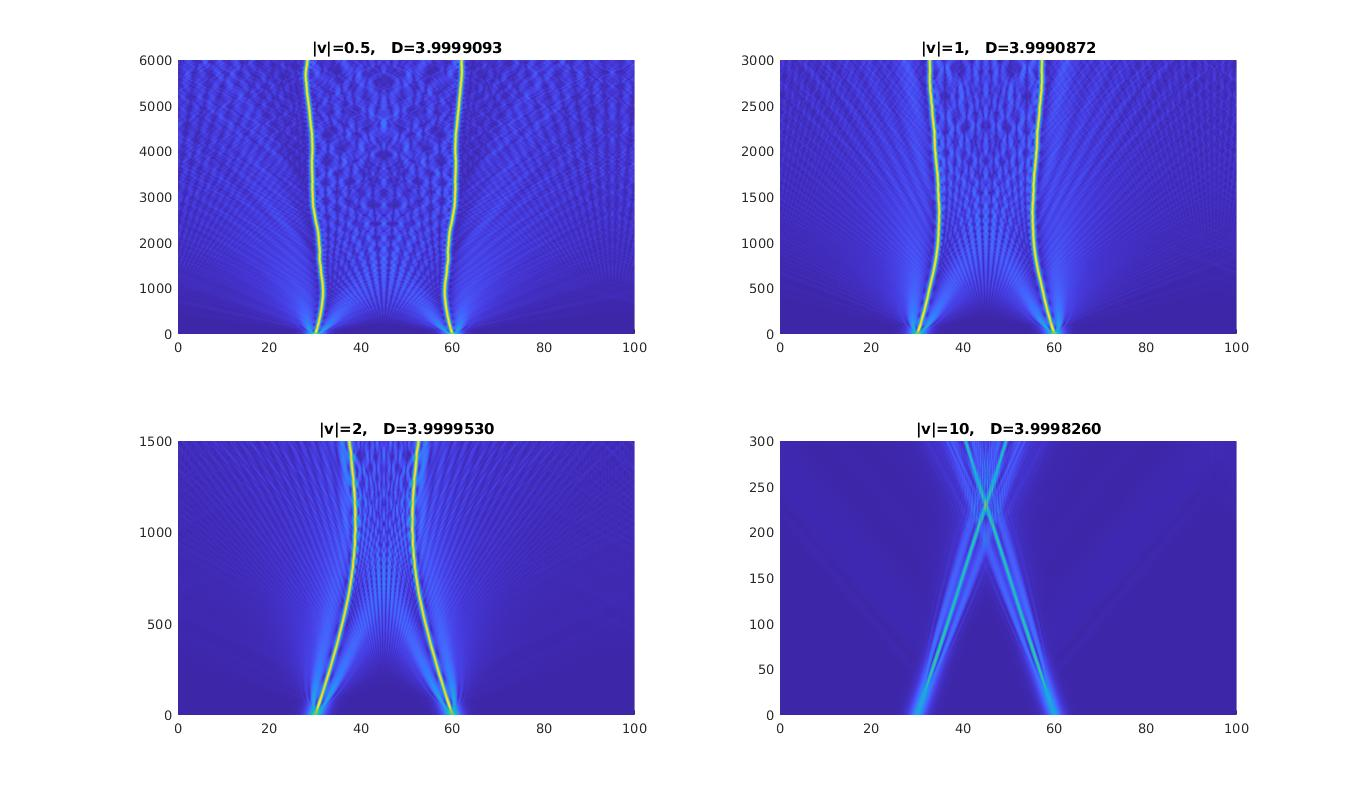
\includegraphics[scale=0.42,center]{3D_V_Sneg09.jpg}
\caption{Above we see some very interesting interactions that once again are reduced by higher velocity}
\end{figure}
In figure 8 we can see that for negative $S$ many small waves form within the medium that interact with each other giving a very distinct pattern. One can also note that for small velocities the solitons do not directly collide but rather seem to deflect with interactions and energy transferred via the smaller interference waves. This effect would be detrimental in information transfer if velocities are small as the initial solitons seem to oscillate and lose velocity, however, information transfer is done using light which has a very high velocity of $2\cdot 10^{8} m/s$ which should reduce these effects dramatically. 
\item Intersoliton distance \\
Figures 9a and 9b show us that intersoliton distance has little effect on the qualitative properties of the collision as 9a shows there is no effect on the simulation (note that the "stretched" effect is due to the different time scales as closer solitons collide in short time).\par
\begin{figure}[h!]
\title{Varying intersolution distance with $S=0$ and $S=0.5$\\}
\subfloat[$S=0$]{
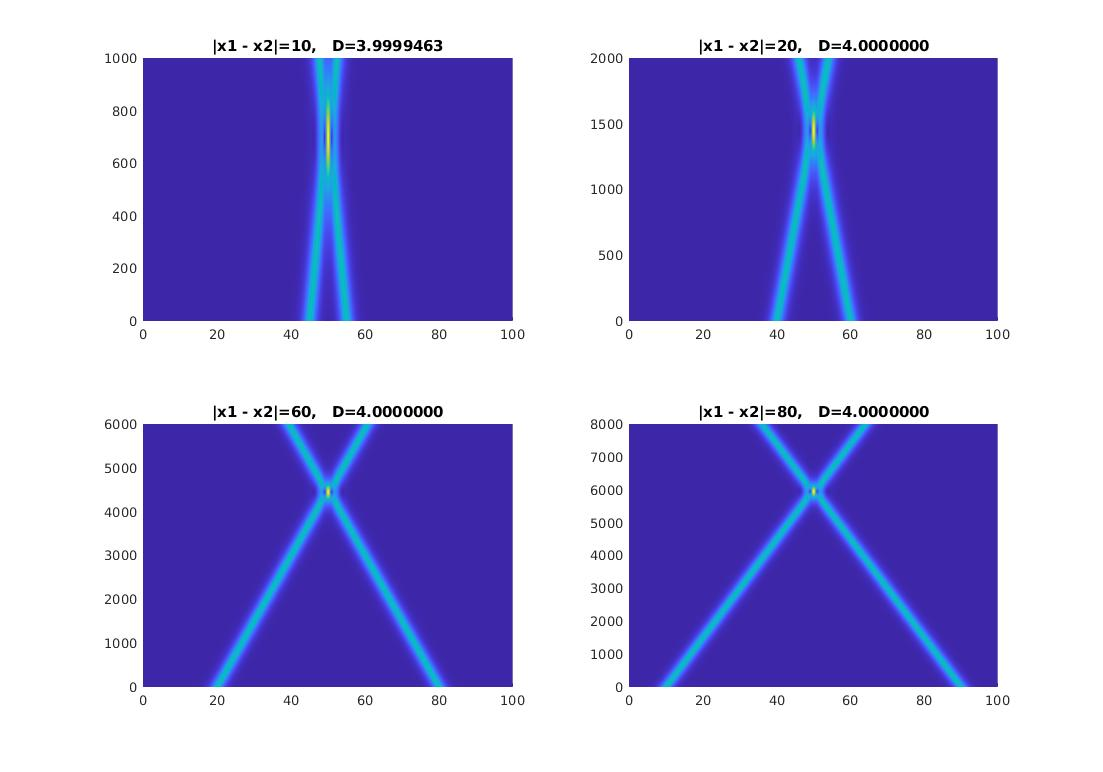
\includegraphics[scale=0.22]{3D_X_S0.jpg}}
\hfill
\subfloat[$S=0.5$]{
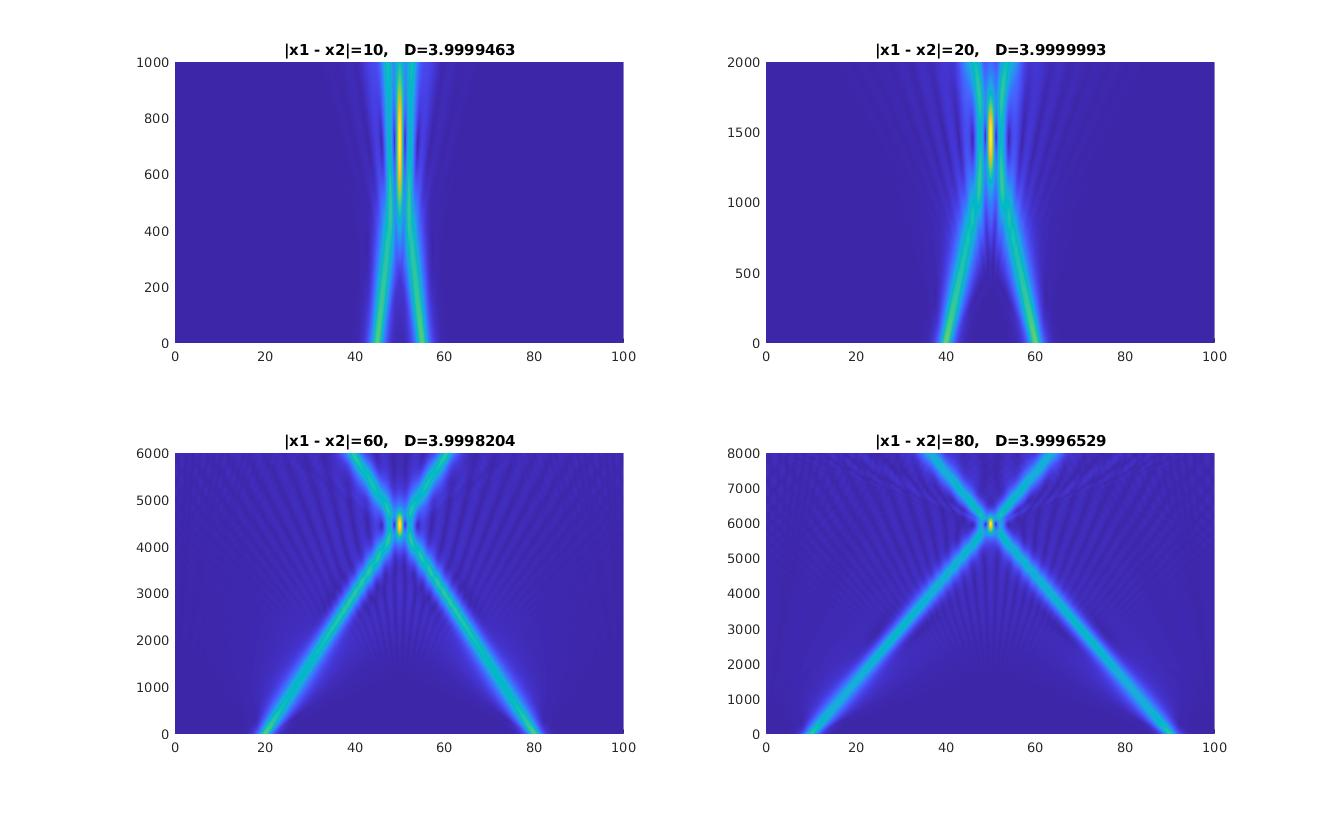
\includegraphics[scale=0.20]{3D_X_S05.jpg}}
\caption{Collision of 2 solions with $v_1=1$ and $v_2=-1$}
\end{figure}
\pagebreak
\begin{figure}
\title{Varying intersoliton distance with $S=-0.5$\\}
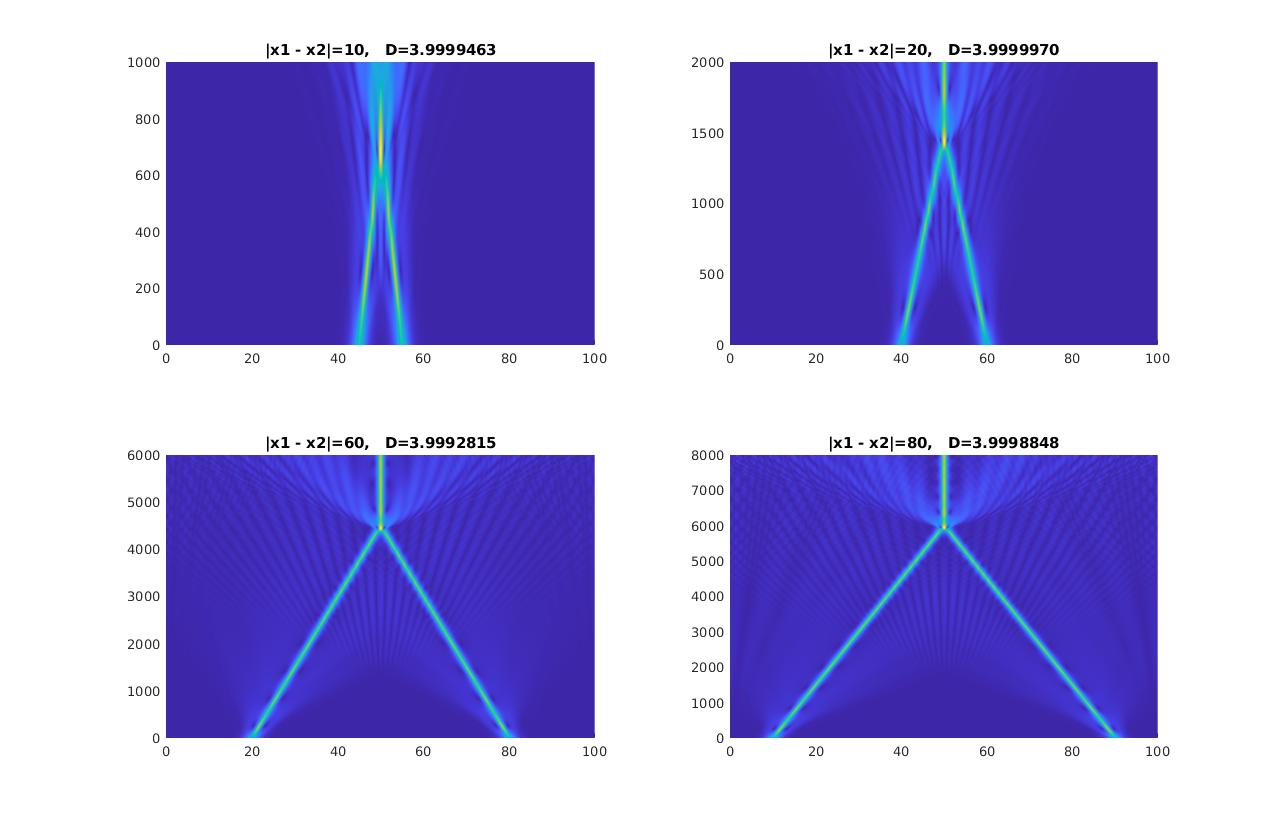
\includegraphics[scale=0.4]{3D_X_Sneg05.jpg}
\caption{Demonstrating standing wave and secondary waves}
\end{figure}
Figure 10 shows us that waves that are sufficiently far apart with negative nonlinear saturation form a standing wave surrounded by interferance. This phenomenon would be detrimental for information transfer as only the secondary interference waves would be transferred in the medium, however, this can be avoided with high enough velocity which is the case for optical waves. \\
Note: That in testing if the intersoliton distance was too small and the value for $N$ or $\tau$ too large numerical errors have a large effect on the simulation, which is resolved by increasing the distance and the simulation ganularity. 
\end{enumerate}
\section{Conclusion}
The numerical analysis of colliding solitons within this paper have indicated several phenomena (Standing waves, secondary waves, spikes and nonelastic collisions). These phenomenon are caused by nonzero values for the nonlinear saturation $S$ which is typical for colliding solitons within optical media. However we discovered that the phenomenon in all cases are reduced if not entirely mitigated by high velocity initial solitons which is the case in optical transmission. The interference (secondary waves) are somewhat of an issue as high velocity waves still produce these artifacts but one can easily mitigate them by calibrating the receivers sensitivity to ignore them, note that there is a chance that superposition of these smaller waves may result in their detection which will need to be corrected in software. \\
The collisions for zero nonlinear saturation were completely elastic with no energy being lost however this was not the case for nonzero values of $S$, this has implications for signal attenuation (signal loss over distance) which may need to be corrected for by some kind of relay to amplify the signal amplitude. \\
Recommendations for further analysis: One should use a numerical method that circumvents the nonintegrability of the Nonlinear Schrodinger equation (1) such as split step to avoid numerical errors effecting results as well as for performance reasons. 

\end{document}